\section{Latency of big blocks with long tails}

Due to operational problems at the production level in case of large
datasets, it may happen that a few files are not produced
properly. They might either be missing (i.e. not even written to
storage) or corrupt with a wrong size/checksum. With the help of
PhEDEx pre/post validation scripts as well as FTS internal mechanisms,
the transfer of these files is reported as a failure back to
PhEDEx. In order to achieve the best throughput in transfers, PhEDEx
puts such failing files back into the transfer queue while
transferring other files, and suspends these transfers for a longer
time when all transfer attempts for a file fail continuously.

The impact of these missing/corrupt files can only be seen in the last
few percentages of the transfer of the whole block. Hence, while
transfer rates in the first 95\% have higher values, rate in the last
5\% drops off to quite low values as shown in the
figure~\ref{fig:figure-5.1}. In a similar way, $RSkewLast_5$
values (see qe.~\ref{eq:revskewlast}) are much lower than
$Skew_{95}$ values (see eq.~\ref{eq:skew}) in
figure~\ref{fig:figure-5.2}.

\begin{figure}[htp]
\centering
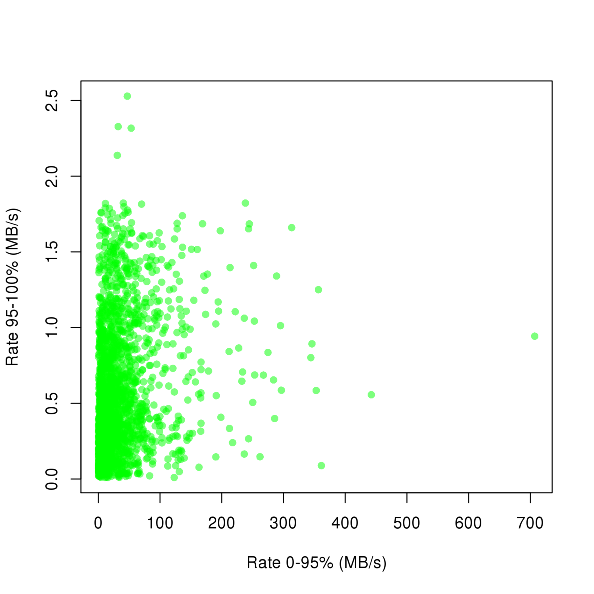
\includegraphics{Figures/figure-51.pdf}
\caption{}\label{fig:figure-5.1}
\end{figure}

\begin{figure}[htp]
\centering
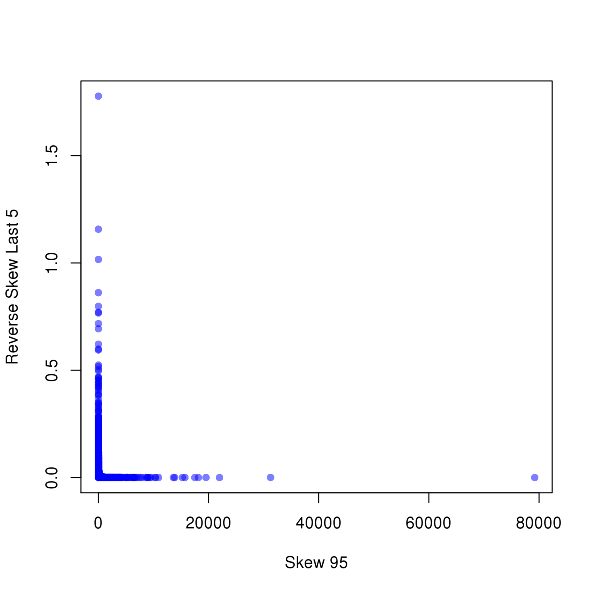
\includegraphics{Figures/figure-52.pdf}
\caption{}\label{fig:figure-5.2}
\end{figure}

When the CMS PhEDEx team investigated the underlying reasons for file
production failures, it was observed that it is mainly due to
transient storage problems. This also explains why only a few files
are affected from this issue. As T1s have more reliable storage
systems, it is mostly T2s that are particularly exposed to this source
of latency, as can be seen in figure~\ref{fig:figure-5.3}.

\begin{figure}[htp]
\centering
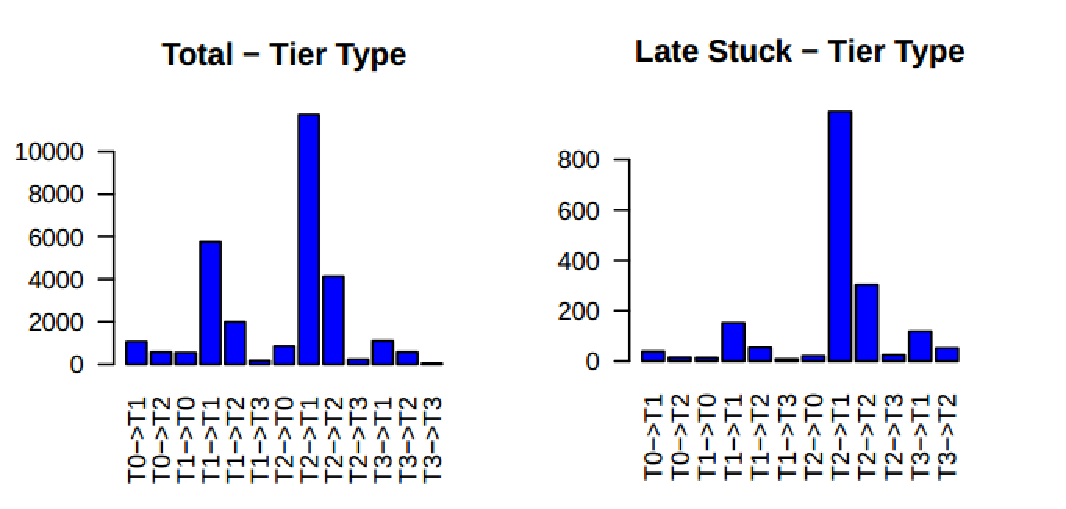
\includegraphics{Figures/figure-53.pdf}
\caption{}\label{fig:figure-5.3}
\end{figure}


Despite the fact that even 99\% of any given sample has already been
transferred to the expected destination, most frequently the
transferred data is useless to CMS jobs until a 100\% transfer
completion is reached. Thus, it is quite important to find the “stuck”
files being the root cause of the latency, and fix the identified
problems as soon as possible. In most cases, solving this problem
requires a manual expert operator intervention, consisting of either
replacing the file (if it has other valid replicas) or otherwise
invalidating it and announcing it as lost.
